% =====================================================================
% Draft 3 SKELETON: "Who Audits the Auditor?"
% Reviewer Heterogeneity and the Social Construction of Privacy-Label Audit.
% Target: International Journal of Human-Computer Studies.
% =====================================================================
\documentclass[11pt,a4paper]{article}

\usepackage[utf8]{inputenc}
\usepackage[T1]{fontenc}
\usepackage{lmodern}
\usepackage{microtype}
\usepackage[margin=2.4cm]{geometry}
\usepackage{graphicx}
\usepackage{xcolor}
\usepackage{booktabs}
\usepackage{array}
\usepackage{caption}
\usepackage{enumitem}
\usepackage{tikz}
\usepackage{pgfplots}
\usepackage{amsmath,amssymb}
\usepackage{url}
\usepackage[hidelinks]{hyperref}
\usepackage[round]{natbib}
\bibliographystyle{plainnat}

\pgfplotsset{compat=1.18}
\usetikzlibrary{arrows.meta,positioning,shapes.geometric,fit,calc,
                patterns,backgrounds,shadows,matrix}

% --- Shared palette
\definecolor{dgBlue}   {RGB}{ 39, 99,178}
\definecolor{dgBlueL}  {RGB}{218,232,248}
\definecolor{dgOrange} {RGB}{226,123, 32}
\definecolor{dgOrangeL}{RGB}{252,229,205}
\definecolor{dgGreen}  {RGB}{ 84,156, 84}
\definecolor{dgGreenL} {RGB}{225,243,217}
\definecolor{dgPurple} {RGB}{132, 76,162}
\definecolor{dgPurpleL}{RGB}{233,221,242}
\definecolor{dgRed}    {RGB}{200, 64, 64}
\definecolor{dgRedL}   {RGB}{248,215,218}
\definecolor{dgTeal}   {RGB}{ 38,140,140}
\definecolor{dgTealL}  {RGB}{211,236,236}
\definecolor{dgGold}   {RGB}{218,165, 32}
\definecolor{dgGoldL}  {RGB}{251,236,196}
\definecolor{dgGrey}   {RGB}{ 90, 90, 90}
\definecolor{dgGreyL}  {RGB}{235,235,235}

\newcommand{\dataguard}{\textsc{DataGuard}}

\title{\bfseries Who Audits the Auditor? \\
Reviewer Heterogeneity and the Social Construction \\
of Privacy-Label Audit}
\author{Anonymous Author(s)\\\small (Skeleton draft for IJHCS submission)}
\date{}

\begin{document}
\maketitle

\begin{abstract}
\noindent\textbf{Skeleton draft.}
Privacy-label audit research typically treats trained reviewers as an
interchangeable population centred on a hidden ground truth. We
re-examine the assumption using the \dataguard{} audit corpus: seven
trained annotators, $1{,}506$ judgments, $1{,}214$ apps. We find a
$15{\times}$ verdict-rate spread (acc~7: $3.2\%$ share-incorrect; acc~6:
$50.1\%$ share-incorrect), a $6{\times}$ evidence-length spread between
the PhD reviewer (median $608$~chars) and the most lenient student
(median $100$~chars), and pair-wise agreement that ranges from $22.7\%$
to $63.6\%$ across annotator pairs. We propose a two-axis reviewer-style
model (vigilance $\times$ engagement) and a reviewer-aware decomposition
of Cohen's $\kappa$ into ambiguity-driven and reviewer-driven
components. The paper argues that privacy audit is a \emph{sociotechnical}
task; design implications cover annotator onboarding, mandatory
evidence pasting and reviewer-weighted aggregation.
\end{abstract}

\noindent\textbf{Keywords:}\ inter-annotator agreement; reviewer effect;
privacy labels; sociotechnical audit; usable privacy.

\bigskip\hrule\bigskip

% =====================================================================
\section{Introduction}
% =====================================================================
\paragraph{Assumption under test.}
Studies that report Cohen's $\kappa$ over a privacy-policy or
privacy-label corpus implicitly treat reviewers as a homogeneous draw
from a population centred on a hidden ground truth. The OPP-115
corpus~\citep{wilson2016creation} reports aggregated agreement across
three legal-trained graduate students but does not analyse the
between-reviewer variance. Crowdsourced annotation studies face the
same issue at scale.

\paragraph{What we find.}
The same task in the same interface produces a $15{\times}$ verdict
spread across seven annotators. This is too large to attribute to
ambiguity alone: the materials are identical, the protocol is identical,
and the interface is identical.

\paragraph{Contribution.}
We propose a two-axis \emph{reviewer-style} model, give a
reviewer-aware decomposition of $\kappa$, and connect both to interface
implications for evidence-grounded audit UIs.

% =====================================================================
\section{Related work}
% =====================================================================
\paragraph{Policy annotation reliability.} OPP-115 and follow-on
work~\citep{wilson2016creation,sathyendra2017identifying,bhatia2016theory}.
\paragraph{Human-AI calibration.} \citet{amershi2019guidelines},
\citet{cai2019hello}, \citet{liao2020questioning}.
\paragraph{Inter-annotator metrics.} \citet{cohen1960coefficient},
\citet{landis1977measurement}.

% =====================================================================
\section{Data}
% =====================================================================
$1{,}506$ judgments from seven annotators with role / age / major /
interest metadata. Account ledger: one PhD-level computer-science
annotator with declared interest in information assurance, six advanced
software-engineering students. Annotators were trained under a fixed
audit protocol; see Draft~$1$ for the interface description.

% =====================================================================
\section{Reviewer-level findings}
% =====================================================================
\subsection{Per-annotator verdict heterogeneity}
Table~\ref{tab:per-ann} reports per-annotator rates for the four
judgment axes. The spread on share-incorrect is from $3.2\%$ (acc~7) to
$50.1\%$ (acc~6); the spread on collect-incomplete is from $6.3\%$
(acc~7) to $79.0\%$ (acc~4).

\begin{table}[t]
\centering\small
\caption{Per-annotator verdict rates.}
\label{tab:per-ann}
\begin{tabular}{lrrrrrr}
\toprule
Acc. & Role & N & \%Inc.share & \%Inc.coll. & \%Incomp.share & \%Incomp.coll.\\
\midrule
1 & PhD/CS/IA      & 172 & 35.5\% & 43.6\% & 43.6\% & 60.5\% \\
2 & SE/.NET        &  63 & 14.3\% & 23.8\% & 15.9\% & 12.7\% \\
3 & SE/AI          &  45 & 33.3\% & 35.6\% &  6.7\% & 22.2\% \\
4 & SE/.NET        & 143 & 32.9\% & 31.5\% & 57.3\% & 79.0\% \\
5 & SE/AI          & 593 & 33.6\% & 31.7\% & 30.0\% & 49.2\% \\
6 & SE/AI          & 427 & 50.1\% & 58.3\% & 29.7\% & 14.1\% \\
7 & SE/IA          &  63 &  3.2\% & 11.1\% &  1.6\% &  6.3\% \\
\bottomrule
\end{tabular}
\end{table}

% --- Figure: per-annotator verdict bars
\begin{figure}[t]
\centering
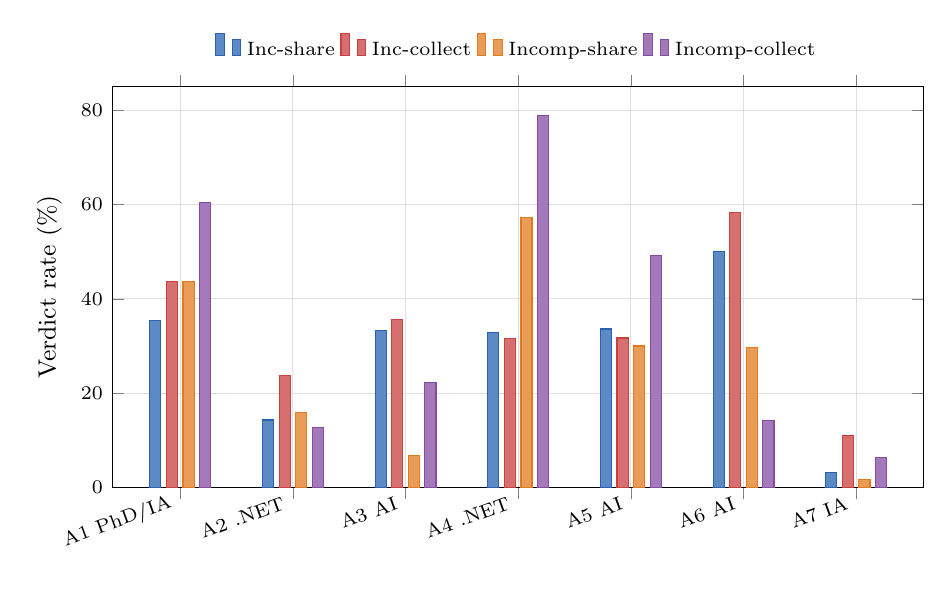
\begin{tikzpicture}
\begin{axis}[
  width=0.98\columnwidth,height=0.55\columnwidth,
  ybar,bar width=4pt,
  ymin=0,ymax=85,
  ylabel={Verdict rate (\%)},
  symbolic x coords={a1,a2,a3,a4,a5,a6,a7},
  xtick=data,
  xticklabels={A1 PhD/IA,A2 .NET,A3 AI,A4 .NET,A5 AI,A6 AI,A7 IA},
  x tick label style={font=\scriptsize,rotate=20,anchor=east},
  legend style={at={(0.5,1.04)},anchor=south,legend columns=4,
                draw=none,font=\scriptsize},
  grid=both,major grid style={draw=gray!25},minor grid style={draw=gray!10},
  tick label style={font=\scriptsize},label style={font=\small}
]
\addplot+[fill=dgBlue!75,draw=dgBlue]   coordinates {
  (a1,35.5)(a2,14.3)(a3,33.3)(a4,32.9)(a5,33.6)(a6,50.1)(a7,3.2)};
\addplot+[fill=dgRed!75,draw=dgRed]     coordinates {
  (a1,43.6)(a2,23.8)(a3,35.6)(a4,31.5)(a5,31.7)(a6,58.3)(a7,11.1)};
\addplot+[fill=dgOrange!75,draw=dgOrange] coordinates {
  (a1,43.6)(a2,15.9)(a3, 6.7)(a4,57.3)(a5,30.0)(a6,29.7)(a7,1.6)};
\addplot+[fill=dgPurple!75,draw=dgPurple] coordinates {
  (a1,60.5)(a2,12.7)(a3,22.2)(a4,79.0)(a5,49.2)(a6,14.1)(a7,6.3)};
\legend{Inc-share,Inc-collect,Incomp-share,Incomp-collect}
\end{axis}
\end{tikzpicture}
\caption{Per-annotator verdict rates across the four judgment axes.
Acc 6 and Acc 7 anchor the high/low ends of vigilance, and Acc 4 and
Acc 6 anchor the high/low ends of completeness perception.}
\label{fig:per-ann-bars}
\end{figure}

\subsection{Engagement: evidence-pasting style}
Table~\ref{tab:ev-len} reports the per-annotator distribution of
evidence-text length pasted into the four \texttt{relevant\_*} fields.

\begin{table}[t]
\centering\small
\caption{Engagement style: pasted-evidence length.}
\label{tab:ev-len}
\begin{tabular}{lrrrr}
\toprule
Acc. & Role & N evidence & Mean (chars) & Median \\
\midrule
1 & PhD     & 535  & 565 & 608 \\
2 & .NET    & 148  & 216 & 160 \\
3 & AI      &  64  & 108 &  99 \\
4 & .NET    & 190  & 202 & 185 \\
5 & AI      & 2083 & 169 & 163 \\
6 & AI      & 1599 & 165 & 152 \\
7 & IA      &   4  & 107 & 100 \\
\bottomrule
\end{tabular}
\end{table}

\paragraph{Reading.} Acc 1 (PhD) pastes evidence that is on average
\emph{three to five times longer} than student annotators. Acc 7
pastes evidence in only $4$ judgments — a near-total absence of evidence
engagement. We treat evidence-length and evidence-presence jointly as
\emph{engagement}.

% =====================================================================
\section{A two-axis reviewer-style model}
% =====================================================================
We plot annotators on two axes:
\emph{vigilance} $= \frac{\#\text{negative verdicts}}{\#\text{total
verdicts}}$,
and \emph{engagement} $= $ median evidence-length pasted.
Four quadrants emerge: high-vigilance high-engagement (PhD, acc~6),
low-vigilance low-engagement (acc~7), high-vigilance low-engagement
(students who flag without explanation), and low-vigilance high-engagement
(rare).

% --- Figure: quadrant
\begin{figure}[t]
\centering
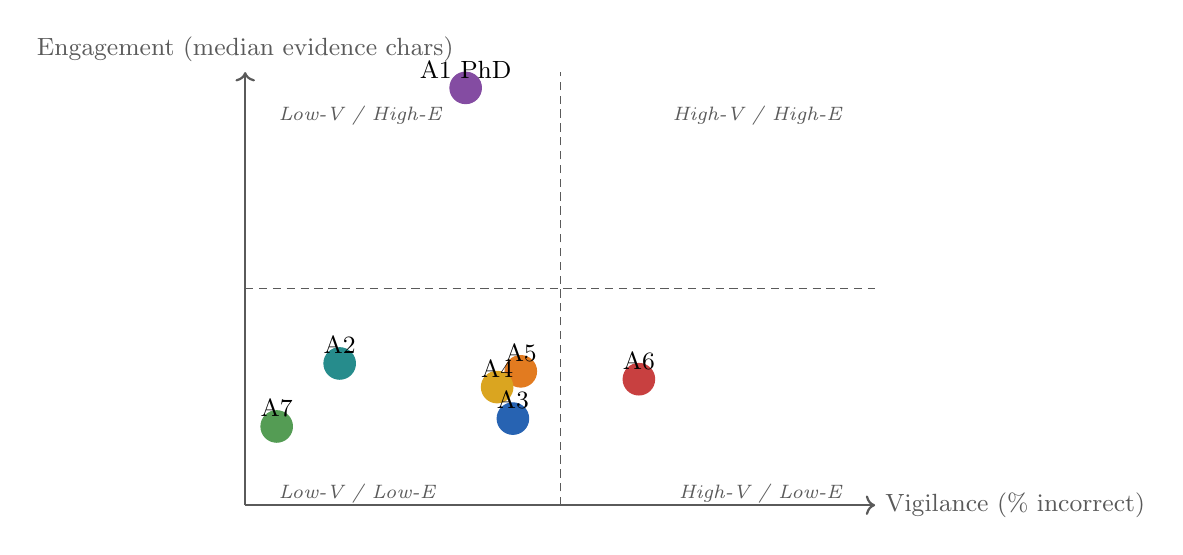
\begin{tikzpicture}[
  every node/.style={font=\small},
  ax/.style={->,thick,dgGrey},
  q/.style={font=\scriptsize\itshape,dgGrey},
  p/.style={circle,fill=dgBlue,minimum size=4mm,inner sep=0pt,draw=dgBlue!70}
]
\draw[ax] (0,0) -- (8,0) node[right]{Vigilance (\% incorrect)};
\draw[ax] (0,0) -- (0,5.5) node[above]{Engagement (median evidence chars)};
\draw[densely dashed,dgGrey] (4,0) -- (4,5.5);
\draw[densely dashed,dgGrey] (0,2.75) -- (8,2.75);
\node[q,anchor=south west] at (0.3,4.7)   {Low-V / High-E};
\node[q,anchor=north west] at (0.3,0.4)   {Low-V / Low-E};
\node[q,anchor=south east] at (7.7,4.7)   {High-V / High-E};
\node[q,anchor=north east] at (7.7,0.4)   {High-V / Low-E};

\node[p,fill=dgPurple,draw=dgPurple]
   at (2.8,5.3) {}; \node[anchor=south] at (2.8,5.3){A1 PhD};
\node[p,fill=dgRed,draw=dgRed]
   at (5.0,1.6) {}; \node[anchor=south] at (5.0,1.6){A6};
\node[p,fill=dgGreen,draw=dgGreen]
   at (0.4,1.0) {}; \node[anchor=south] at (0.4,1.0){A7};
\node[p,fill=dgOrange,draw=dgOrange]
   at (3.5,1.7) {}; \node[anchor=south] at (3.5,1.7){A5};
\node[p,fill=dgTeal,draw=dgTeal]
   at (1.2,1.8) {}; \node[anchor=south] at (1.2,1.8){A2};
\node[p,fill=dgGold,draw=dgGold]
   at (3.2,1.5) {}; \node[anchor=south] at (3.2,1.5){A4};
\node[p,fill=dgBlue,draw=dgBlue]
   at (3.4,1.1) {}; \node[anchor=south] at (3.4,1.1){A3};
\end{tikzpicture}
\caption{Two-axis reviewer-style model. The PhD anchors high engagement;
acc 7 anchors low everything. Vigilance and engagement are only weakly
correlated.}
\label{fig:quadrant}
\end{figure}

\subsection{Pairwise agreement matrix}
We report the symmetric pair-wise agreement matrix below.
Table~\ref{tab:pairwise} reports the five most data-rich pairs.

\begin{table}[t]
\centering\small
\caption{Most data-rich pairs by shared-app count.}
\label{tab:pairwise}
\begin{tabular}{lrrr}
\toprule
Pair & shared apps & Agree share & Agree collect \\
\midrule
(A1, A5) & 85  & 49.4\% & 52.9\% \\
(A1, A6) & 11  & 45.5\% & 63.6\% \\
(A2, A3) & 14  & 50.0\% & 57.1\% \\
(A5, A6) & 156 & 48.1\% & 50.6\% \\
(A5, A7) & 22  & 22.7\% & 40.9\% \\
\bottomrule
\end{tabular}
\end{table}

% =====================================================================
\section{Reviewer-aware \texorpdfstring{$\kappa$}{kappa}}
% =====================================================================
\paragraph{Sketch.} Decompose pairwise $\kappa$ into:
$\kappa = \kappa_{\text{ambig}} + \kappa_{\text{style}}$
where $\kappa_{\text{style}}$ is the agreement loss attributable to
divergent marginal verdict rates between the two annotators (their
expected-agreement floors differ) and $\kappa_{\text{ambig}}$ is the
residual ambiguity in the materials. We compute the decomposition for the
five pairs in Table~\ref{tab:pairwise}.

% =====================================================================
\section{Design implications}
% =====================================================================
\paragraph{R1 Calibration tasks at onboarding.} Before a reviewer is
counted, run them on a fixed gold subset and report their style on the
two axes; surface the result back to the reviewer.
\paragraph{R2 Mandatory evidence for negative verdicts.}
The interface should require an evidence paste for any \emph{Incorrect}
or \emph{Incomplete} judgment, matching the PhD's de facto practice.
\paragraph{R3 Reviewer-weighted aggregation.}
When multiple reviewers vote on an app, weight them by their style
profile rather than averaging blind.

% =====================================================================
\section{Discussion, limitations, conclusion}
% =====================================================================
\paragraph{Limitations.} Seven annotators is a small sample;
$n = 11$ for pair (A1,A6) limits some pair-wise tests; annotators are
not a representative reviewer pool.
\paragraph{Conclusion.} Reviewer style is a measurable property of
privacy-label audit. Treating it as residual noise overstates the
ambiguity of the materials and understates the design responsibility
of the audit interface.

\bibliography{../draft-01-auditability-gap/references}

\end{document}
